	\subsection{Sous-mission A2}
	\begin{vwcol}[widths={0.65,0.2}, rule=0pt]
		\begin{minipage}{0.7\textwidth}
			\paragraph{Objectifs de la mission}

			Déterminer la quantité de méthane dans l'atmosphère de la planète Mars, afin de déterminer si il y a une présence de vie sur cette planète. Pour se faire nous avions à disposition une photographie satellite de la surface de Mars.
		\end{minipage}

		\begin{minipage}{0.3\textwidth}
			\begin{flushright}
				\paragraph{Techniques utilisées}
			
				Proportion \&
				Moyenne
			\end{flushright}
		\end{minipage}
	\end{vwcol} 

	\begin{figure}[h]
		\centering
		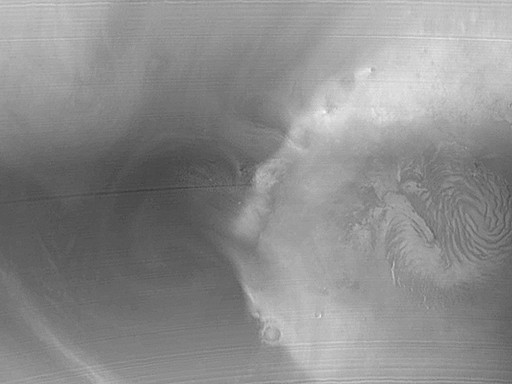
\includegraphics[scale=0.6]{images/Mars_surface.png}
	\end{figure}
	\vspace{-0.3cm}

	\paragraph{Procédé}	
		Pour remplir la mission nous avons calculé le taux de pixel, puis fais la somme des taux des pixels. Enfin, nous avons fait la moyenne du taux de gaz afin de déterminer la quantité de gaz dans l'atmosphère martienne. Nous n'avons pas eu besoin d'utiliser des filtres.